\documentclass[border=6pt]{standalone}
\usepackage{amsmath,amssymb}
\usepackage{tikz}
\usetikzlibrary{arrows.meta}
\begin{document}
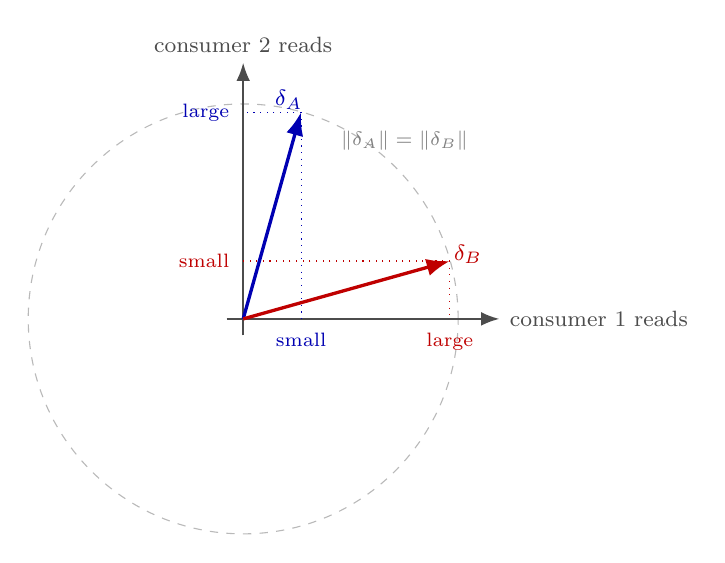
\begin{tikzpicture}[>=Latex,scale=1.05]
  \draw[gray!55,dashed] (0,0) circle (2.6);
  \draw[->,thick,black!70] (-0.2,0)--(3.1,0) node[right,font=\footnotesize]{consumer 1 reads};
  \draw[->,thick,black!70] (0,-0.2)--(0,3.1) node[above,font=\footnotesize]{consumer 2 reads};
  % equal-norm error vectors (|dA|=|dB|=2.6)
  \draw[->,very thick,blue!70!black] (0,0)--(0.7,2.5);
  \node[blue!70!black,font=\footnotesize] at (0.55,2.65){$\delta_A$};
  \draw[->,very thick,red!75!black] (0,0)--(2.5,0.7);
  \node[red!75!black,font=\footnotesize] at (2.72,0.78){$\delta_B$};
  % projections onto consumer-1 axis
  \draw[blue!70!black,dotted] (0.7,2.5)--(0.7,0);
  \draw[red!75!black,dotted]  (2.5,0.7)--(2.5,0);
  \node[blue!70!black,font=\scriptsize,anchor=north] at (0.7,-0.05){small};
  \node[red!75!black,font=\scriptsize,anchor=north] at (2.5,-0.05){large};
  % projections onto consumer-2 axis
  \draw[blue!70!black,dotted] (0.7,2.5)--(0,2.5);
  \draw[red!75!black,dotted]  (2.5,0.7)--(0,0.7);
  \node[blue!70!black,font=\scriptsize,anchor=east] at (-0.05,2.5){large};
  \node[red!75!black,font=\scriptsize,anchor=east] at (-0.05,0.7){small};
  \node[gray,font=\scriptsize] at (1.95,2.15){$\|\delta_A\|=\|\delta_B\|$};
\end{tikzpicture}
\end{document}
